\section{Introductie}
Elke na zomer slippen de grachten van Delft dicht met kroos. Kroos is een familie van planten die zich niet wortelen in de bodem. Kroos drijft met blaadjes, de grootte varieert erg per soort, op het wateroppervlak. Kroos kan goed bloeien in stil staand water. Algen kunnen juist beter bloeien in stromend water. Waaronder grote open water lichamen zoals de Noordzee of oceanen. Hier hebben algen een moordende invloed. Een plaag van algen of kroos kan veroorzaakt worden door een overschot aan nutriënten, wat kan ontstaan door bijvoorbeeld overbemesting. Bij een overschot aan nutriënten zoals stikstof en fosfaten is er geen concurrentie meer over deze stoffen. Hierdoor kunnen algen exponentieel groeien. Een dichte algen[Hey Hey HEY wil je even naar de chat kijken? Groetje Billy vanuit het vliegtuig] -laag kan zorgen voor het tegenhouden van licht en zuurstof. Door het gebrek aan licht zullen andere planten afsterven, waardoor het zuurstof gehalte van het water nog verder afneemt. Zonder zuurstof in het water zullen vissen en andere organismen niet meer kunnen overleven. Het eco-systeem zal bijna helemaal uitsterven. Dit proces heet eutrofiëring. Net zoals in Figuur \ref{fig:bloom} zijn er over de hele wereld lichamen van water die uitsterven. De bacteriën die algen verteren verbruiken in het geval van een plaag alle zuurstof in het water. Deze bacteriën kunnen ook enorm toe nemen in populatie omdat er zo veel algen zijn. Veel onderzoek is gewijd aan het voorspellen en voorkomen van zulke plagen. \\
Aan de kern van ons onderzoek ligt het verslag van \cite{Algen1985}, hier wordt een algemeen model beschreven om algen te modelleren. Sinds 1985 is er extreem veel ingewikkeld en uitgebreider onderzoek bij gekomen. Om dit verslag simpel te houden wordt echter het door \cite{Algen1985} model aangehouden. Dit model is gegeven als een differentiaal vergelijking. Om dit op te lossen wordt de Runge-Kutta 4 integratie methode toegepast, in Python. Er zal geanalyseerd worden wanneer dit stabiel gebeurd voor het gereduceerde model. We zullen dit model uitbreiden met 1 ruimtelijke coördinaat door hier een stroming en diffusie deel aan toe te voegen. In \cite{Algen1985} wordt ook een fotosynthetische-snelheid geïmpliceerd, deze zal hier verder uitgewerkt worden. \textbf{Uiteindelijk blab blab bla}
\begin{figure}[H]
    \centering
    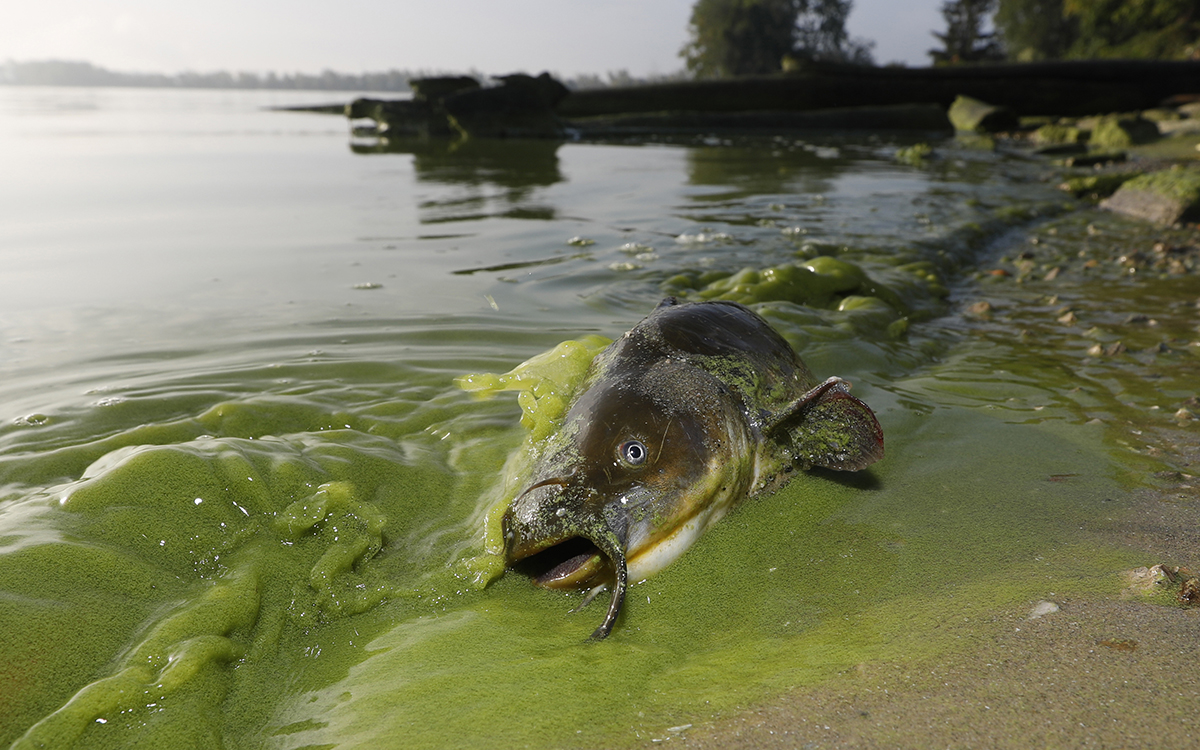
\includegraphics[width=0.6\textwidth]{figures/Algbloom.jpg}
    \caption{Water gevuld door algen in North Toledo, OHIO (US) | PHOTO BY ANDY MORRISON/THE BLADE VIA AP PHOTO}
    \label{fig:bloom}
\end{figure}
